\subsection{Classical Multidimensional Scaling (cMDS)}
\label{subsec:cMDS}

Classical multidimensional scaling (cMDS) is a technique used to visualize the distances between entities in a lower-dimensional space, typically two or three dimensions. Unlike Principal Component Analysis (PCA), which aims to maximize data variation, cMDS focuses on preserving the original distances between points as accurately as possible. This approach is detailed in Chapter 6 of Wang (2012) \cite{wangClassicalMultidimensionalScaling2012}.
Your section on Classical Multidimensional Scaling (cMDS) is clear and well-structured. Below is a refined version to enhance rigor, flow, and conciseness.

Given a set of \( n \) entities represented by a distance matrix \( D = [d_{ij}]_{i,j=1}^{n} \), cMDS seeks a configuration \( \mathcal{Y} = \{y_1, \ldots, y_n\} \) in \( \mathbb{R}^d \) such that the Euclidean distances \( d_{\mathcal{Y}}(y_i, y_j) \) between points \( y_i \) and \( y_j \) in \( \mathcal{Y} \) approximate the original distances \( d_{ij} \):

\begin{equation}
    d_{\mathcal{Y}} (y_i, y_j) \approx d_{ij}, \quad \forall i, j.
    \label{eq:cmds-approximation}
\end{equation}

First, the distance matrix \( D \) is centered using the centering matrix \( H = I - \frac{1}{n} \mathbf{1} \mathbf{1}^T \), where \( I \) is the identity matrix and \( \mathbf{1} \) is a vector of ones. The centered Gram matrix \( G^C \) is calculated as:

\begin{equation}
    G^C = -\frac{1}{2} H D^2 H,
    \label{eq:cmds-gram-matrix}
\end{equation}
where \( D^2 \) is the element-wise square of the distance matrix \( D \). Next, eigendecomposition is performed on \( G^C \) to obtain its eigenvalues \( \lambda_i \) and corresponding eigenvectors \( u_i \):

\begin{equation}
    G^C = U \Sigma U^T,
    \label{eq:cmds-eigen-decomposition}
\end{equation}
where \( U = [u_1, u_2, \ldots, u_r] \) and \( \Sigma = \text{diag}(\lambda_1, \lambda_2, \ldots, \lambda_r) \). The eigenvalues and eigenvectors are sorted in descending order of the eigenvalues. To construct the configuration matrix \( Y \), the top \( d \) eigenvalues and their corresponding eigenvectors are selected. Let \( U_d = [u_1, u_2, \ldots, u_d] \) and \( \Sigma_d = \text{diag}(\sqrt{\lambda_1}, \sqrt{\lambda_2}, \ldots, \sqrt{\lambda_d}) \). The configuration matrix \( Y \) is then given by:

\begin{equation}
    Y = U_d \Sigma_d.
    \label{eq:cmds-configuration-matrix}
\end{equation}

For visualization, the first two columns of \( Y \) are typically plotted to provide a two-dimensional representation of the data.


%%%%%%%%%%%%%%%%%%%%%%%%%%%%%%%%%%%%%%%%%%%%%%%%%%%%%%%%%%%%

By applying cMDS to the distance matrices generated by the reparameterization search at depth 10 and logarithmic signature truncation at level 3, the motion capture data can be visualized in two dimensions. This visualization is performed for both the original distances and the reduced distances obtained by PCA combined with cosine similarity. The cluster assignments obtained by K-Medoids clustering are included to better understand the data structure. The original reparameterization with clustering is shown in Figure \ref{fig:2d-reparameterization-depth10}, the reduced reparameterization with clustering in Figure \ref{fig:2d-reparameterization-depth10_reduced}, the original logarithmic signature with clustering in Figure \ref{fig:2d-logsig-level3}, and the reduced logarithmic signature with clustering in Figure \ref{fig:2d-logsig-level3_reduced}.

The figures demonstrate that the clustering utilizing the reparameterization method is quite distinct, especially when colored by the true cluster assignments. The reduced data show even clearer cluster formations in the 2D space, with the reduced clustering numbers more aligned with the true cluster assignments.

In the logarithmic signature method, the data are not as distinct as in the reparameterization method, for both the original and reduced data. However, the reduced data still show clearer cluster formations in 2D space.

In the reduced reparameterization data, "forward jump", "run/jog" and "walk" are distinct, while "boxing" and "climbing stairs" are somewhat mixed but still relatively distinct. For the logarithmic signature method, only "forward jump" is clearly separate, while "run/jog", "walk" and "climbing stairs" are somewhat distinct, with "boxing" mixed with the other clusters. This suggests that the "boxing" movement may resemble other movements, making it less distinct.

Overall, these results indicate that distinguishing real motion capture data using these methods is feasible. The application of post-processing techniques such as PCA with cosine distance, cMDS, and clustering enhances the clarity of the results compared to the heatmap figures \ref{fig:heatmaps-dynprog}, \ref{fig:heatmaps-logsig}.

\begin{figure}
    \centering
    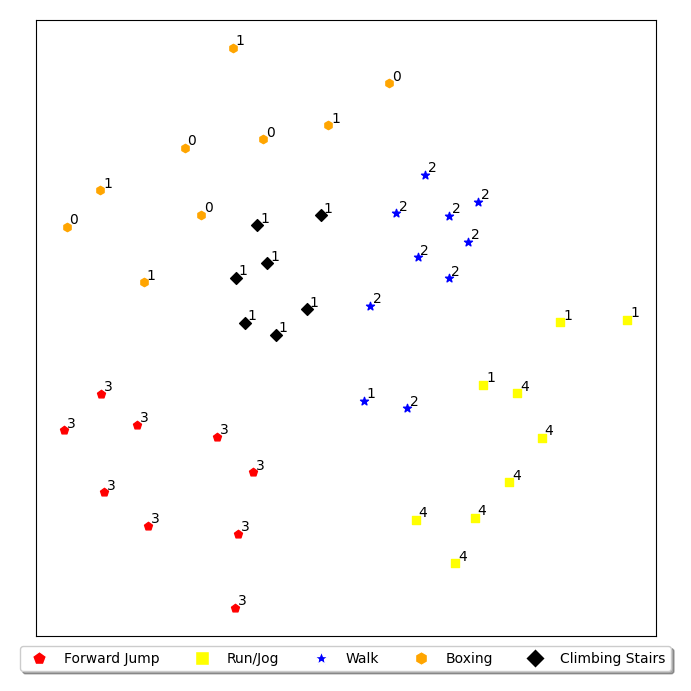
\includegraphics[width=0.99\textwidth]{figures/motion-capture-data/2d_plots/reparameterization_depth10}
    \caption[2D cMDS Visualization of Reparameterized Motion Capture Data (Search Depth 10)]{2D visualization using cMDS of the reparameterization of motion capture data with dynamic programming using search depth 10. Colors and shapes represent the true cluster assignments, while the numbers indicate cluster assignments generated by K-Medoids clustering, with five clusters.}
    \label{fig:2d-reparameterization-depth10}
\end{figure}

\begin{figure}
    \centering
    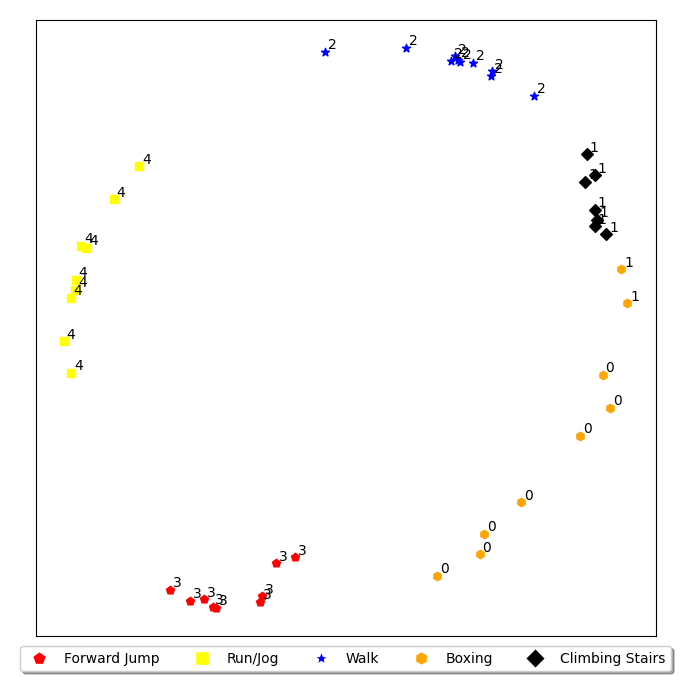
\includegraphics[width=0.99\textwidth]{figures/motion-capture-data/2d_plots/reparameterization_depth10_red}
    \caption[2D cMDS Visualization of PCA-Reduced Reparameterized Motion Capture Data (Search Depth 10)]{2D visualization using cMDS of the reduced reparameterization of motion capture data, reduced to 4 dimensions using PCA and rebuilt with cosine distance, with dynamic programming using search depth 10. Colors and shapes represent the true cluster assignments, while the numbers indicate cluster assignments generated by K-Medoids clustering, with five clusters.}
    \label{fig:2d-reparameterization-depth10_reduced}
\end{figure}

\begin{figure}
    \centering
    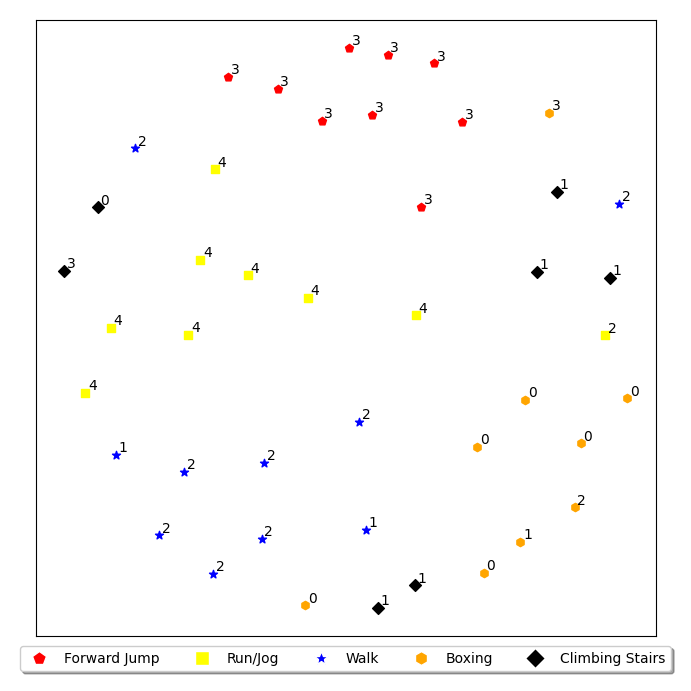
\includegraphics[width=0.99\textwidth]{figures/motion-capture-data/2d_plots/logsig_level3}
    \caption[2D cMDS Visualization of Logarithmic Signature Motion Capture Data (Truncation Level 3)]{2D visualization using cMDS of the logarithmic signature of motion capture data with truncation level 3. Colors and shapes represent the true cluster assignments, while the numbers indicate cluster assignments generated by K-Medoids clustering, with five clusters.}
    \label{fig:2d-logsig-level3}
\end{figure}

\begin{figure}
    \centering
    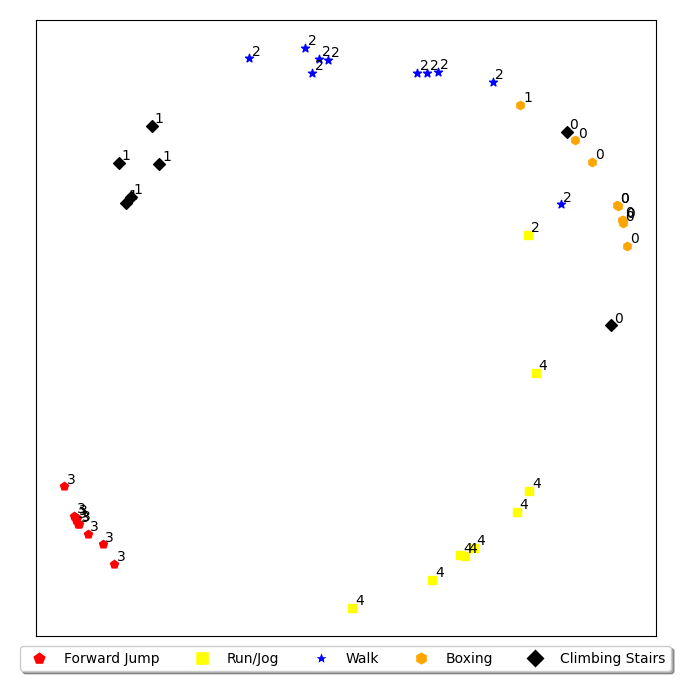
\includegraphics[width=0.99\textwidth]{figures/motion-capture-data/2d_plots/logsig_level3_red}
    \caption[2D cMDS Visualization of PCA-Reduced Logarithmic Signature Motion Capture Data (Truncation Level 3)]{2D visualization using cMDS of the reduced logarithmic signature of motion capture data, reduced to 4 dimensions using PCA and rebuilt with cosine distance, with truncation level 3. Colors and shapes represent the true cluster assignments, while the numbers indicate cluster assignments generated by K-Medoids clustering, with five clusters.}
    \label{fig:2d-logsig-level3_reduced}
\end{figure}
